\scanpage{58}
\[
u_r:\widetilde{\mathcal G}_3\xrightarrow{\sim}\widetilde{\mathcal G}_3
\]
et tout repère $r'$ \inserted{\unsure{au $=$ $\varepsilon$ pour $r$|avec $=$ $\varepsilon$ pour $r$}} sera de la forme de façon unique
\[
r'=rg_0\quad\text{avec }g_0\in\widetilde{\mathcal G}_3
\]
\[
(38)\quad\text{i.e.}\quad u_{r'}=u_ru_{g_0}\qquad(\text{avec }u_r(g_0)=g\text{ mais peu importe})
\]
d'où, en passant à l'action sur les $\Pi_1$ en $P_+$ resp. $P_\varepsilon$, on trouve
\[
(39)\qquad \psi_{r'\deleted{\unsure{\varepsilon}}}=\psi_r\circ\Pi_1(g_0,P_+)\qquad\text{si }r'=r\circ g_0.
\]
\margin{$\psi_r,\psi_{r'}$ désignent ici les isoms. d'épinglage associés \deleted{aux} à $P_\varepsilon$.}
On va expliciter ceci pour
\[
g_0=\rho\quad\text{donc }r'=r\rho=(\omega i,\omega,\bar\omega)\quad\text{si }r=(i,\omega,\bar\omega)
\]
On trouve
\[
\psi_\varepsilon^{\omega i,\omega}=\inserted{\rho_\omega\circ\psi_\varepsilon^{i,\omega}=}\psi_\varepsilon^{i,\omega}\circ\rho
\]
où on a identifié $\rho$ aussi à un élément de $\widetilde\Pi_{0,3}$, et à l'autom qu'il induit sur $\Pi_{0,3}$.

\uline{NB} $\rho_\omega$ est la rotation autour de $P_\varepsilon,P_{\varepsilon'}$ d'un tiers de tour, \deleted{\unsure{suivant}} l'orientation $\omega$ sur l'équateur.

\margin{\uline{NB}\quad $\psi_\varepsilon^{i,\omega}(l_0),\psi_\varepsilon^{i,\omega}(l_1),\deleted{\unsure{\psi_\varepsilon^{i,\omega}(l_0)}}$ sont resp. les lacets \unsure{standart|standard} à partir de $P_\varepsilon$, autour des trous $R_{\omega i},R_{\omega^2i}$, \deleted{\unsure{qui}} passant $Q_i$ (donc \unsure{au détriment de} $\unsure{R_{\omega\prime i}|R_{\omega i}}$ : $R_{\omega i}\cdots$), et dans le sens d'orientation $\bar\omega=\omega\wedge\varepsilon$.}
\figure{
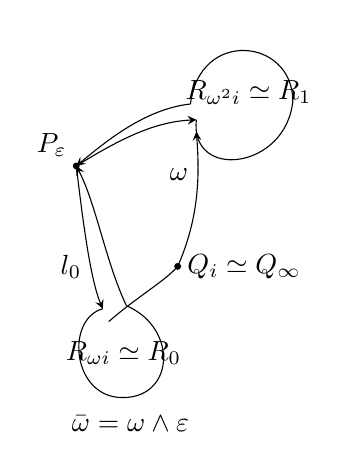
\begin{tikzpicture}[scale=1.25,>=stealth]
\coordinate (p) at (0,1.2);\coordinate (q) at (1.03,.18);
\fill (p) circle(1pt) node[above left]{$P_\varepsilon$};
\fill (q) circle(1pt) node[right]{$Q_i\simeq Q_\infty$};
\draw[->] (p) .. controls (.06,.7) and (.14,.05) .. (.27,-.25) node[pos=.65,left]{$l_0$};
\draw (.27,-.25) .. controls (-.1,-.35) and (-.05,-1.1) .. (.42,-1.15) .. controls (1,-1.2) and (1.05,-.45) .. (.51,-.22);
\draw[->] (.51,-.22) .. controls (.3,.22) and (.2,.82) .. (p);
\draw[->] (p) .. controls (.45,1.48) and (.8,1.65) .. (1.22,1.67);
\draw (1.22,1.67) .. controls (1.15,1.05) and (2.13,1.16) .. (2.2,1.86) .. controls (2.2,2.5) and (1.25,2.6) .. (1.16,1.83);
\draw[->] (1.16,1.83) .. controls (.7,1.78) and (.3,1.45) .. (p);
\draw (.33,-.38) .. controls (.63,-.12) and (.9,.03) .. (q);
\draw[->] (q) .. controls (1.26,.7) and (1.25,1.15) .. (1.22,1.55) node[pos=.65,left]{$\omega$};
\node at(.48,-.7){$R_{\omega i}\simeq R_0$};
\node at(1.75,1.95){$R_{\omega^2i}\simeq R_1$};
\node[below]at(.55,-1.24){$\bar\omega=\omega\wedge\varepsilon$};
\end{tikzpicture}}
On trouve de $=$, pour un autom qui renverse l'orientation de $\sigma$, i.e. pour un
\[
\widetilde\sigma_\infty:\quad\begin{array}{rcl}0&\longrightarrow&1\\1&\longrightarrow&0\\\infty&\longrightarrow&\infty\end{array}\qquad\deleted{\unsure{la}\ \illegible{1}}\bar\omega\longmapsto\bar\omega'
\]
\deleted{$\unsure{\widetilde\sigma_\infty}$}
\[
g_0=\widetilde\sigma_\infty\qquad r'=r\sigma_\infty=(\deleted{\unsure{\omega}}i,\omega',\bar\omega').
\]
d'où
\[
(41)\qquad\psi_\varepsilon^{\deleted{\unsure{\omega}}i,\omega'}=\inserted{\widetilde\sigma_i\circ\psi_\varepsilon^{i,\omega}=}\psi_\varepsilon^{i,\omega}\circ\widetilde\sigma_\infty
\]
($\widetilde\sigma_i$ est la symétrie p.r. du grand cercle méridien passant par $Q_i$)
\margin{57}

